% !TEX root = ../../main.tex
% !TEX spellcheck = en_US
\section{Evaluation and experimentation methods}
To evaluate our bot (and later our hypothesis) we conducted three evaluations and a final experimentation. The first evaluation was in the design phase of the bot. Here we asked StarCraft players on forums\footnote{
Team Liquid: \url{http://www.teamliquid.net/forum/viewmessage.php?topic_id=308630}\\
Battle.net: \url{http://eu.battle.net/sc2/en/forum/topic/3312961916} accessed 2012-09-03.} what they would like to see in a teammate bot.
%: Write about what features they would like to see.
\marginpar{write about features}

Close to when BATS was finished the authors played with it find remaining bugs and minor improvements that could be made. When the majority of the bugs was fixed, an additional tester evaluated the bot’s control and behavior to find further improvements that were needed before the final experiment.

\paragraph{Player evaluation}
From the player evaluation we conducted that an improvement needed to be made to how commands were send. For one available commands weren’t visible to the player, but s/he had to remember them. This gave the idea to create GUI buttons for the player client. These can be seen in figure \ref{fig:player_commands_gui}

\begin{figure}[htb]
\centering
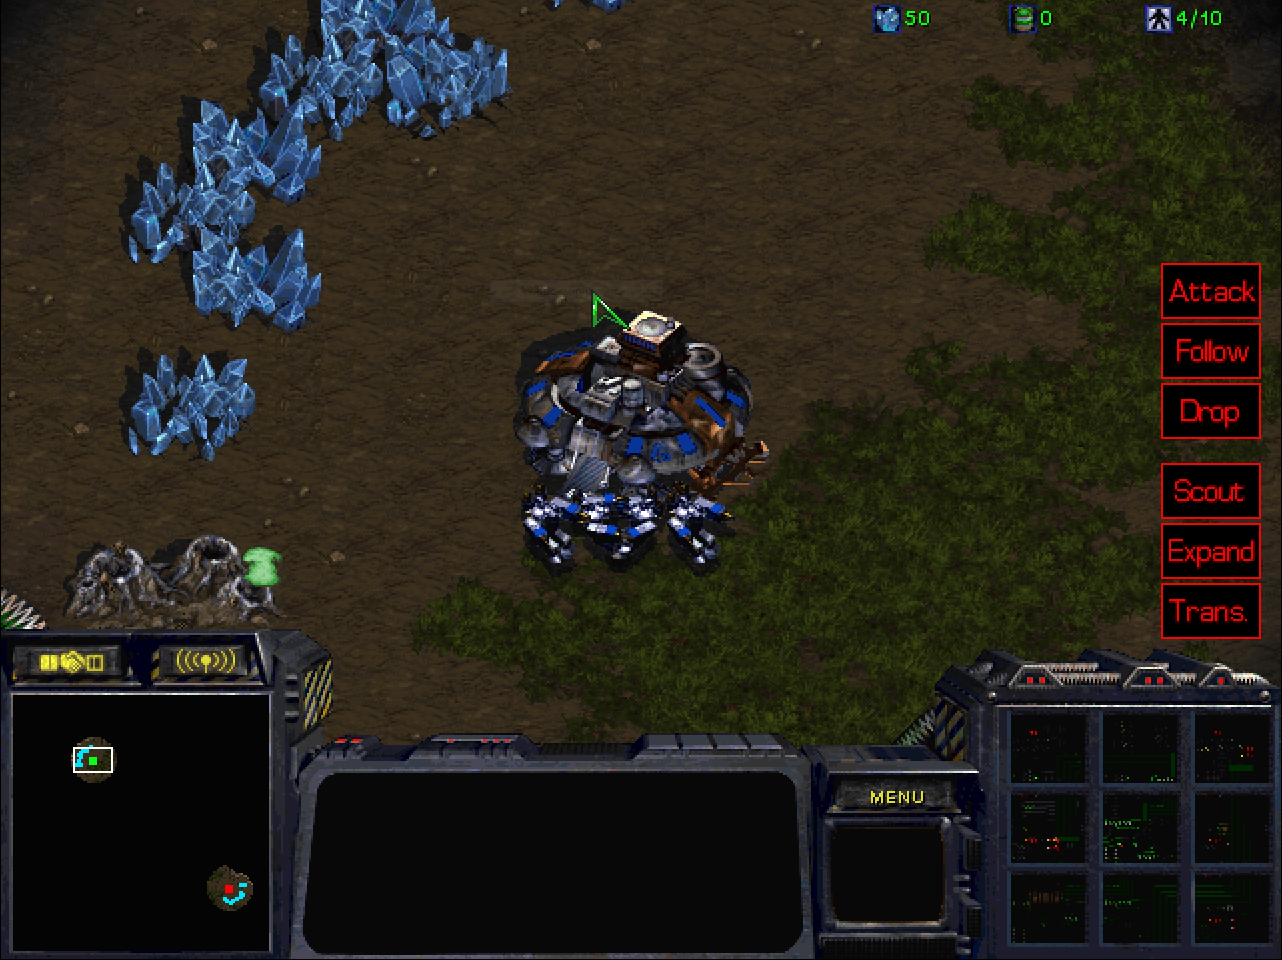
\includegraphics[width=0.8\textwidth]{player_gui_controls}
\caption{Player client with GUI commands enabled}
\label{fig:player_commands_gui}
\end{figure}

\subsection{Experiment method}
The experiment is divided in three parts, first the player preparation where the player would play skirmish matches against the default AI to refresh his/her skills or familiarize him-/herself with StarCraft and the map, the experiment will be conducted on. This could be done a couple of days before the experiment to the same day the experiment was, depending on the tester’s preferences.

The second part was the actually experiment itself. Here the player was presented with four scenarios he would play.
\begin{inparaenum}[1\upshape)]
	\item No control over the bot and the bot would not communicate its intentions;
	\item With control over bot, but no communication;
	\item With communication, but no control; and
	\item With both control and communication enabled.
\end{inparaenum}
To \h1{avoid a scenario preference depending} on the orders, the testers will use a different ordering of the scenarios. This will, however, have a side effect: Tester that start with both communication and control might be overwhelmed with both having a teammate and the need to check it’s intention messages and be able to control it.

The scenarios are played at fastest game speed, both because normal speed is slow (the experiment would be too long) and it is considered a standard to play at fastest game speed in the StarCraft community, although the campaign is played at normal game speed. Each scenario had a limit to 20 minutes because the testers could otherwise have played hour-long scenarios. If the player is winning after 20 minutes, the tester was asked if we should speed up the game or close it—the matches were sped up to roughly 10 times faster speed (depending on computer speed), thus the game usually ended within a minute or two. This was done to let the player win for the experiment to continue to be interesting.
